\documentclass[aspectratio=169,xcolor=dvipsnames]{beamer}
\usetheme{SimpleDarkBlue}

\usepackage{hyperref}
\usepackage{graphicx}
\usepackage{booktabs}
\usepackage{inconsolata} 

\title[Mark -- AI Investment Assistant]{Mark -- Your Personal AI Investment Assistant}
\author{Ciro Francesco Amabile, Vincenzo Carbone, Gerardo D'Arco}
\date{}

\begin{document}

% Slide 1: Title
\frame{\titlepage}

% Slide 2: Introduction
\begin{frame}{Introduction}
  Our goal is to create a virtual financial assistant capable of answering questions about publicly traded companies.\\
  \vspace{0.1cm}
  
  To ensure that the data is always up to date, we plan to use a \textbf{VPS (Virtual Private Server)}, where the pipeline will run periodically using \texttt{crontab}.
  
  \vspace{0.1cm}
  Mark is powered by a \textbf{RAG (Retrieval-Augmented Generation)} pipeline that combines:
  \begin{itemize}
      \item \textbf{Retrieval:} the system searches the financial data for the most relevant content related to the user's question
      \item \textbf{Augmented Generation:} the retrieved content is used as context to generate an accurate answer with an advanced language model (GPT)
  \end{itemize}
  
  \vspace{0.1cm}
  In summary, Mark combines:
  \begin{itemize}
      \item Collected and cleaned financial data
      \item NLP techniques for semantic understanding
      \item GPT models for clear and professional answers
  \end{itemize}
\end{frame}
  

% Slide 3: Project Structure
\begin{frame}{Project Structure}
  \centering
  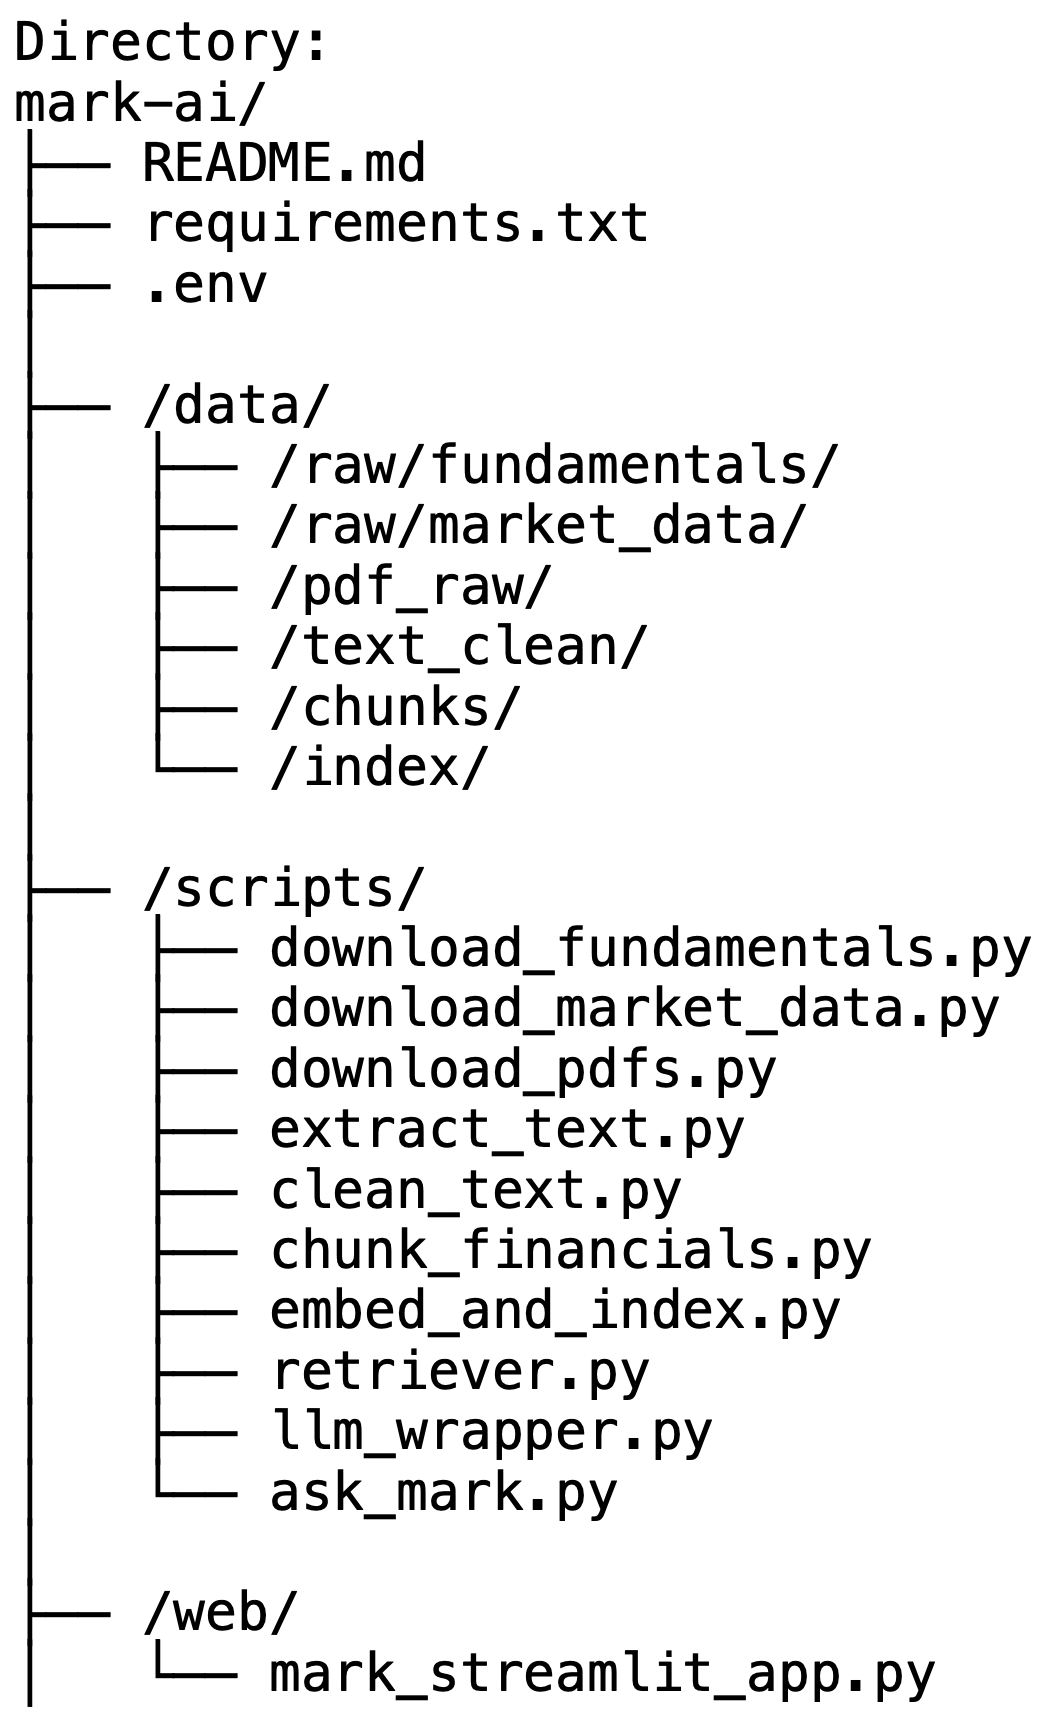
\includegraphics[width=0.33\linewidth]{directory.png}
  \end{frame}
  
% Slide 4: Project Structure - In Depth
\begin{frame}{Project Structure - In Depth}
  \textbf{Main directory: mark-ai/}
  
  \vspace{0.2cm}
  \begin{itemize}
      \item \texttt{data/} \\
      Contains all raw and processed data. Subdivided into:
      \begin{itemize}
          \item \texttt{raw/fundamentals}, \texttt{raw/market\_data}: data downloaded via API
          \item \texttt{pdf\_raw}: company PDFs obtained via web scraping
          \item \texttt{text\_clean}: cleaned and formatted text extracted from PDFs
          \item \texttt{chunks}: information blocks ready for embedding
          \item \texttt{index}: FAISS vector database and mapping
      \end{itemize}
  
      \item \texttt{scripts/} \\
      Contains all Python scripts for the pipeline. Each file performs a specific function: scraping, cleaning, embedding, retrieval, and response generation.
  
      \item \texttt{web/} \\
      Future upgrade for a web-based user interface.
  
      \item \texttt{README.md, requirements.txt, .env} \\
      Support files: project documentation, required libraries, and environment variables (e.g., API keys).
  \end{itemize}
\end{frame}
  
% Slide 5: Data - Collection and Cleaning (Detailed)
\begin{frame}{Data: Collection and Cleaning}
  \textbf{1. Automated data collection:}
  \begin{itemize}
      \item We use \texttt{yfinance} to obtain:
      \begin{itemize}
          \item \textbf{Fundamental data}: revenue, net income, P/E ratio, operating margin, ROE, etc.
          \item \textbf{Market data}: current price, historical prices, beta, trading volumes
      \end{itemize}
      \item Outputs are saved as \texttt{.json} or \texttt{.csv} files in the \texttt{data/raw/} directory
      \item In parallel, we can download \textbf{PDFs} (quarterly reports, ESG documents, press releases) via web scraping from official websites (Investor Relations, SEC, CONSOB)
  \end{itemize}
  
  \vspace{0.2cm}
  \textbf{2. Cleaning and pre-processing:}
  \begin{itemize}
      \item Conversion of numbers and percentages into standardized formats
      \item Removal of noise from text (page numbers, repeated headers, unwanted symbols)
      \item Normalization of content to ensure consistency across different sources
      \item Production of "clean" text ready for chunk segmentation
  \end{itemize}
\end{frame}

% Slide 6: Scripts - Detailed Overview
\begin{frame}{Scripts - Detailed Overview}
  \textbf{1. Data Collection}
  \begin{itemize}
      \item \texttt{download\_fundamentals.py}: downloads key variables (revenue, income, P/E, etc.)
      \item \texttt{download\_market\_data.py}: retrieves stock prices, trading volumes, beta, etc
  \end{itemize}
  
  \textbf{2. PDFs and Text}
  \begin{itemize}
      \item \texttt{download\_pdfs.py}: scrapes PDFs from official company websites
      \item \texttt{extract\_text.py}: extracts raw text from the downloaded PDFs
      \item \texttt{clean\_text.py}: cleans and normalizes the extracted content
  \end{itemize}
  
  \textbf{3. Chunk Preparation}
  \begin{itemize}
      \item \texttt{chunk\_financials.py}: segments the text into semantic blocks ("chunks") with metadata
  \end{itemize}
  
  \textbf{4. Embedding and Indexing}
  \begin{itemize}
      \item \texttt{embed\_and\_index.py}: generates numerical embeddings and creates a FAISS index
  \end{itemize}
  
  \textbf{5. User Interaction}
  \begin{itemize}
      \item \texttt{retriever.py}: retrieves the most relevant chunks for the given question
      \item \texttt{llm\_wrapper.py}: builds the prompt and calls the ChatGPT API
      \item \texttt{ask\_mark.py}: CLI script that allows direct interaction with Mark
  \end{itemize}
\end{frame}

% Slide 7: Embedding and FAISS - In Depth
\begin{frame}{Embedding and FAISS}
  \textbf{1. Semantic Embedding}
  \begin{itemize}
      \item Each \textbf{text chunk} (300–500 words) is transformed into a high-dimensional \textbf{numerical vector} that captures its meaning.
      \item We use OpenAI’s \texttt{text-embedding-ada-002} model, one of the most efficient and semantically accurate models available.
      \item Result: each information block becomes a set of numbers that reflects its semantic essence.
  \end{itemize}
  
  \vspace{0.3cm}
  \textbf{2. FAISS (Facebook AI Similarity Search)}
  \begin{itemize}
      \item The vectors are stored and indexed in a \textbf{vector store} using the \texttt{FAISS} library, designed for fast similarity search across millions of vectors.
      \item When a user submits a question, it is also embedded into a vector.
      \item The system compares this vector with all chunk vectors and retrieves the most semantically similar ones.
  \end{itemize}
\end{frame}

% Slide 8: Final expected Output
\begin{frame}{Final expected Output}
  \textbf{Example user question:} \\
  \texttt{"What is Apple's P/E ratio and how does it compare to Microsoft's?"}
  
  \vspace{0.4cm}
  \textbf{1. Retrieval of relevant chunks}
  \begin{itemize}
      \item The system converts the question into a vector embedding.
      \item Using FAISS, it retrieves the most semantically similar chunks (e.g., data on Apple and Microsoft).
  \end{itemize}
  
  \vspace{0.2cm}
  \textbf{2. Prompt construction}
  \begin{itemize}
      \item The selected chunks are formatted as "context" for GPT.
      \item A structured prompt is built, including both the relevant data and the user's question.
  \end{itemize}
  
  \vspace{0.2cm}
  \textbf{3. Answer generation}
  \begin{itemize}
      \item The GPT-3.5/4 model analyzes the information and generates a clear, professional answer.
      \item Output: a comparison of the P/E ratios, with possible comments on high/low values and market implications.
  \end{itemize}
\end{frame}
  

% Slide 9: Scalability - Future Extensions
\begin{frame}{Scalability: Future Extensions}
  The project is designed to be easily scalable. Potential extensions include:
  
  \vspace{0.05cm}
  \textbf{1. Integration with new data sources}
  \begin{itemize}
      \item Expanding data sources via \textbf{APIs} (e.g., Bloomberg)
      \item Automated \textbf{web scraping} to collect data from financial portals, Investor Relations pages, and open-access databases
  \end{itemize}
  
  \textbf{2. Market sentiment analysis}
  \begin{itemize}
      \item Scraping of news and articles to perform \textbf{sentiment analysis}, useful for anticipating market reactions to events or announcements
  \end{itemize}
  
  \textbf{3. Regulatory analysis and legal transparency}
  \begin{itemize}
      \item Extraction of content from public institutional sources to generate responses that also reflect the \textbf{rights and obligations} of a fully informed investor
  \end{itemize}
  
  \textbf{4. New user interfaces}
  \begin{itemize}
      \item Integration with a \textbf{Telegram bot} for quick queries
      \item Development of a \textbf{web dashboard} using Streamlit or FastAPI
  \end{itemize}

\end{frame}

  

% Slide 10: Final Thanks (Centered Title)
\begin{frame}

  \centering
  {\LARGE \textbf{Thank you for your attention!}}
  
  \vspace{0.8cm}
  
  \textbf{Project developed by:}
  
  \vspace{0.3cm}
  \begin{itemize}
      \item Ciro Francesco Amabile
      \item Vincenzo Carbone
      \item Gerardo D'Arco
  \end{itemize}
  
  \vspace{0.6cm}
  \textit{“Investing is no longer just about numbers — it's about automated intelligence.”}
  
  \end{frame}
  

\end{document}
